% CVPR 2026 Paper Template; see https://github.com/cvpr-org/author-kit

\documentclass[10pt,twocolumn,letterpaper]{article}

%%%%%%%%% PAPER TYPE  - PLEASE UPDATE FOR FINAL VERSION
\usepackage[pagenumbers]{cvpr} % camera-ready layout with page numbers
% \usepackage{cvpr}              % To produce the CAMERA-READY version
% \usepackage[review]{cvpr}      % To produce the REVIEW version

% Import additional packages in the preamble file, before hyperref
%% This file contains a number of tweaks that are typically applied to the main document.
%% They are not enabled by default, but can be enabled by uncommenting the relevant lines.

%%
%% Inline annotations; for predefined colors, refer to "dvipsnames" in the xcolor package:
%% https://tinyurl.com/overleaf-colors
%%
\newcommand{\red}[1]{{\color{red}#1}}
\newcommand{\todo}[1]{{\color{red}#1}}
\newcommand{\TODO}[1]{{\color{gray}#1}}  % gray hint: what to write here
%%
%% disable for camera ready / submission by uncommenting these lines  
%%
% \renewcommand{\TODO}[1]{}
% \renewcommand{\todo}[1]{#1}

%%
%% work harder in optimizing text layout. Typically shrinks text by 1/6 of page, enable
%% it at the very end of the writing process, when you are just above the page limit
%%
% \usepackage{microtype}

%%
%% fine-tune paragraph spacing
%%
% \renewcommand{\paragraph}[1]{\vspace{.5em}\noindent\textbf{#1.}}

%%
%% globally adjusts space between figure and caption
%%
% \setlength{\abovecaptionskip}{.5em}


%%
%% Allows "the use of \paper to refer to the project name"
%% with automatic management of space at the end of the word
%%
% \usepackage{xspace}
% \newcommand{\paper}{ProjectName\xspace}

%%
%% Commonly used math definitions
%%
% \DeclareMathOperator*{\argmin}{arg\,min}
% \DeclareMathOperator*{\argmax}{arg\,max}

%%
%% Tigthen underline
%%
% \usepackage{soul}
% \setuldepth{foobar}

%%
%% Lab3 additions
%%
\usepackage{array}   % m{} columns: vertically centered image grids
\usepackage{listings}
\lstset{language=Python, basicstyle=\ttfamily\scriptsize, columns=fullflexible,
        breaklines=true, frame=single, keywordstyle=\color{NavyBlue}\bfseries,
        commentstyle=\color{gray}, showstringspaces=false}

%% \img[width]{path}: a framed placeholder box (path label scaled to fit) until the image file exists;
%% raised to sit on the baseline like a real image, so row labels center the same way
\newcommand{\img}[2][\linewidth]{\IfFileExists{#2}{\includegraphics[width=#1]{#2}}{%
  \raisebox{\depth}{\fbox{\parbox[c][\dimexpr#1-2\fboxsep-2\fboxrule][c]{\dimexpr#1-2\fboxsep-2\fboxrule}{\centering
  \resizebox{\linewidth}{!}{\parbox{2cm}{\centering\tiny\def\UrlBreaks{\do\/\do\_}\nolinkurl{#2}}}}}}}}
\newcolumntype{C}[1]{>{\centering\arraybackslash}m{#1}}

%% Images live in Figure/: Figure/{sds,vsd,sdi}/<prompt>.png, Figure/ablation/<setting>/<value>/<prompt>.png
%% \resrow{method dir}{row label}: one row with all 10 evaluation prompts
\newcommand{\resrow}[2]{\rotatebox{90}{\scriptsize #2}
  & \img{Figure/#1/A_red_bus_driving_on_a_desert_road.png} & \img{Figure/#1/a_boat_in_a_river.png}
  & \img{Figure/#1/A_cabin_surrounded_by_forests.png}      & \img{Figure/#1/A_church_beside_a_lake.png}
  & \img{Figure/#1/A_villa_close_to_the_pool.png}          & \img{Figure/#1/A_castle_next_to_a_river.png}
  & \img{Figure/#1/A_burger_on_the_table.png}              & \img{Figure/#1/A_dog_sitting_on_grass.png}
  & \img{Figure/#1/a_cat_sitting_on_a_table.png}           & \img{Figure/#1/A_car_on_the_road.png} \\}

%% \ablpanel{setting}{5 values}: value labels on top, then 3 labeled prompts (rows) x 5 values (columns)
%% \ablcell: ablation image size; Fig. 6 uses 1.5\ablcell, so its 2 rows are as tall as the 3 ablation rows
\newlength{\ablcell}\setlength{\ablcell}{.087\textwidth}
\newcommand{\ablrow}[8]{\rotatebox{90}{\scriptsize #3} & \img{Figure/ablation/#1/#4/#2.png} & \img{Figure/ablation/#1/#5/#2.png}
  & \img{Figure/ablation/#1/#6/#2.png} & \img{Figure/ablation/#1/#7/#2.png} & \img{Figure/ablation/#1/#8/#2.png} \\}
\newcommand{\ablpanel}[6]{%
  \begin{tabular}{@{}m{1em}*{5}{C{\ablcell}}@{}}
    & \scriptsize #2 & \scriptsize #3 & \scriptsize #4 & \scriptsize #5 & \scriptsize #6 \\
    \ablrow{#1}{A_burger_on_the_table}{Burger}{#2}{#3}{#4}{#5}{#6}
    \ablrow{#1}{a_cat_sitting_on_a_table}{Cat}{#2}{#3}{#4}{#5}{#6}
    \ablrow{#1}{A_villa_close_to_the_pool}{Villa}{#2}{#3}{#4}{#5}{#6}
  \end{tabular}}


\definecolor{cvprblue}{rgb}{0.21,0.49,0.74}
\usepackage[pagebackref,breaklinks,colorlinks,allcolors=cvprblue]{hyperref}

\def\paperID{*****}
\def\confName{CVPR}
\def\confYear{2026}

%%%%%%%%% TITLE
\title{Lab3-Score Distillation Sampling Implementation}

%%%%%%%%% AUTHORS
\author{Your Name (Student ID)\\
NYCU\\
{\tt\small your.email@example.com}
}

\begin{document}
\twocolumn[{%
\renewcommand\twocolumn[1][]{#1}%
\maketitle
\begin{center}
  \captionsetup{type=figure}
  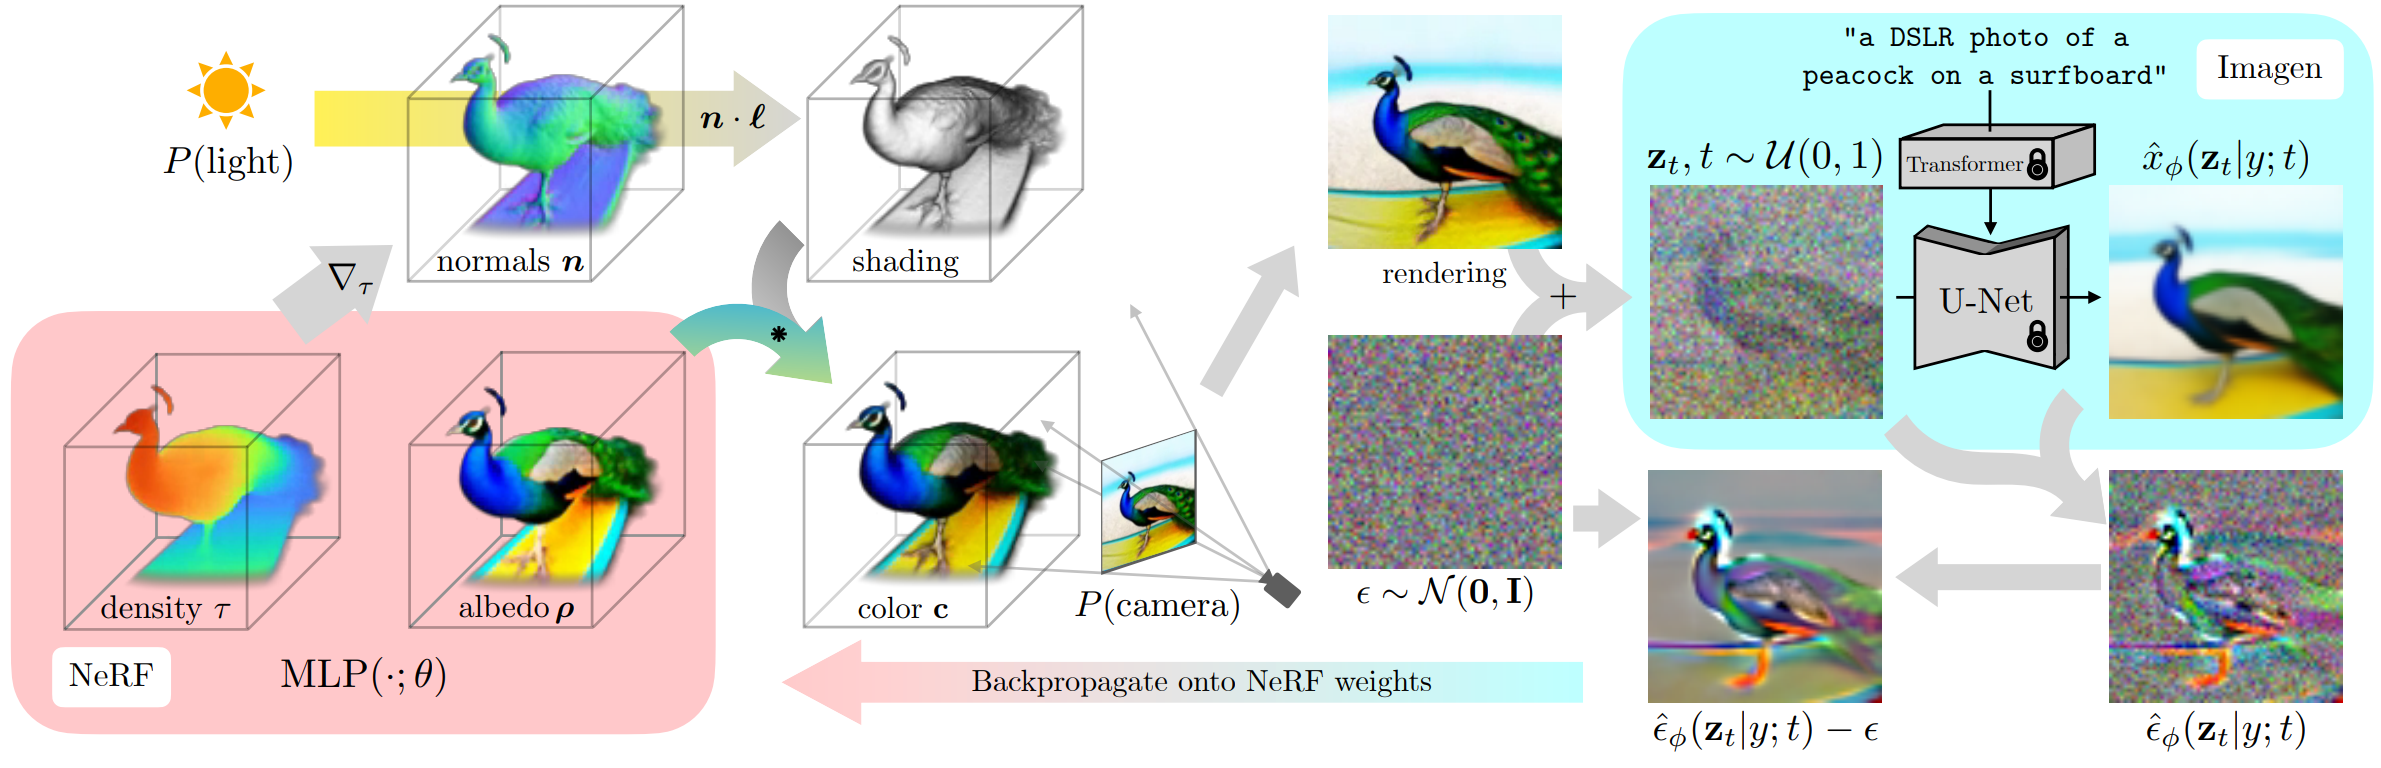
\includegraphics[width=\textwidth]{Figure/1_teaser.png}
  \captionof{figure}{\textbf{Overview of score distillation.} A rendered image is noised and scored by a frozen text-to-image diffusion model, and the residual $\hat\epsilon_\phi - \epsilon$ is backpropagated to the 3D parameters. In this lab the 3D representation is replaced by a 2D latent. Figure from DreamFusion~\cite{poole2023dreamfusion}.}
  \label{fig:teaser}
\end{center}
\vspace{1em}
}]
  % \maketitle + teaser figure
\section{Introduction}
\label{sec:intro}
% [2 pts] Briefly describe and summarize the goal of this assignment.

Ordinary diffusion sampling starts from pure noise and runs the reverse process step by step to produce an image.
Score distillation instead treats the image (here, a Stable Diffusion latent) as a set of free parameters and uses a frozen, pretrained diffusion model only as a \emph{critic}: at every iteration the model looks at a noisy version of the current latent and tells us in which direction it should move to look more like the text prompt.
This turns a diffusion model into a loss function, which is what makes text-to-3D methods such as DreamFusion~\cite{poole2023dreamfusion} possible (\cref{fig:teaser}).

In this assignment I implemented three score distillation methods on top of Stable Diffusion 2.1-base for text-to-image generation:
Score Distillation Sampling (SDS)~\cite{poole2023dreamfusion},
Variational Score Distillation (VSD)~\cite{wang2023prolificdreamer}, and
Score Distillation via Inversion (SDI)~\cite{lukoianov2024sdi}.
Each method optimizes a $1\times4\times64\times64$ latent for the 10 evaluation prompts, and the results are evaluated with the CLIP ViT-B/32 image--text similarity~\cite{radford2021clip}.
I also ran the required ablations on the SDS guidance scale and on the SDI inversion steps and update interval, and an extra experiment with the original diffusion loss.

\Cref{sec:method} describes the methods and my implementation, \cref{sec:exp} reports the results and ablations, and \cref{sec:discussion} discusses why the plain diffusion loss fails and why VSD and SDI improve over SDS.

\section{Methodology}
\label{sec:method}
% [6 pts] Explain SDS, VSD, and SDI; both the concept and your implementation.

\noindent\textbf{Background.}
All three methods share the same frozen Stable Diffusion UNet $\epsilon_\theta(x_t, y, t)$~\cite{rombach2022ldm}, which predicts the noise in a noisy latent $x_t$ given a prompt $y$ and timestep $t$.
The forward process~\cite{ho2020ddpm} produces $x_t = \sqrt{\bar\alpha_t}\,x_0 + \sqrt{1-\bar\alpha_t}\,\epsilon$ with $\epsilon\sim\mathcal N(0, I)$.
Noise predictions use classifier-free guidance (CFG)~\cite{ho2022cfg}, $\hat\epsilon_\theta = \epsilon_{\text{uncond}} + s\,(\epsilon_{\text{cond}} - \epsilon_{\text{uncond}})$, where the unconditional branch uses the negative prompt ``low quality''.
The optimized parameter is the latent $x_0$, initialized from $\mathcal N(0, I)$ and decoded with the VAE only for visualization.
The optimizer (AdamW, cosine schedule, gradient clipping) is the one provided in \texttt{main.py}.

%-------------------------------------------------------------------------
\subsection{Score Distillation Sampling (SDS)}
\label{sec:sds}

\noindent\textbf{Concept.}
SDS~\cite{poole2023dreamfusion} noises the current latent with a random $t$ and $\epsilon$, asks the diffusion model to predict the noise, and uses the difference as the update direction:
$\nabla_{x_0} L_{\text{SDS}} = w(t)\,(\hat\epsilon_\theta(x_t, y, t) - \epsilon)$.
Intuitively, the residual $\hat\epsilon_\theta - \epsilon$ points from the current image towards what the model thinks a clean image for this prompt looks like.
This is the gradient of the ordinary diffusion loss with the UNet Jacobian term dropped; skipping it makes SDS cheap (no backpropagation through the UNet) and, as \cref{sec:diff_loss} shows, is also what makes it work at all.

\noindent\textbf{Implementation.}
I sample $t\sim\mathcal U[20, 980]$ and $\epsilon$, add noise with the scheduler, and predict the noise with CFG under \texttt{no\_grad}.
The gradient uses the DreamFusion weight $w(t)=1-\bar\alpha_t$.
To feed this hand-made gradient to the optimizer, I write it as an MSE to a detached target $x_0 - \text{grad}$, whose derivative with respect to $x_0$ is exactly the SDS gradient.

\begin{lstlisting}
def get_sds_loss(self, latents, text_embeddings, guidance_scale=7.5):
    B = latents.shape[0]
    t = torch.randint(self.min_step, self.max_step + 1, (B,), device=self.device)
    noise = torch.randn_like(latents)
    with torch.no_grad():
        latents_noisy = self.scheduler.add_noise(latents, noise, t)
        noise_pred = self.get_noise_preds(latents_noisy, t, text_embeddings, guidance_scale)
    w = (1 - self.alphas[t]).view(B, 1, 1, 1)
    grad = torch.nan_to_num(w * (noise_pred - noise))
    # d(loss)/d(latents) == grad (skips the UNet Jacobian)
    target = (latents - grad).detach()
    return 0.5 * F.mse_loss(latents, target, reduction="sum") / B
\end{lstlisting}

%-------------------------------------------------------------------------
\subsection{Variational Score Distillation (VSD)}
\label{sec:vsd}

\noindent\textbf{Concept.}
In SDS the reference $\epsilon$ is pure random noise, so the update is noisy and SDS needs a very large guidance scale to converge, which causes over-smoothed and over-saturated results.
VSD~\cite{wang2023prolificdreamer} replaces $\epsilon$ with the prediction of a second network $\epsilon_\phi$, a LoRA~\cite{hu2022lora} on top of the same UNet, which is trained online to model the distribution of the images currently being generated.
The update $w(t)\,(\hat\epsilon_\theta - \epsilon_\phi)$ then compares ``what the pretrained model expects'' with ``what we currently generate'', which is a much cleaner signal and works with a normal guidance scale of 7.5.

\noindent\textbf{Implementation.}
The LoRA (rank 4 on the attention projections) is set up by the provided code.
For $\epsilon_\theta$ I temporarily disable the adapters and predict with CFG; for $\epsilon_\phi$ I enable them and use only the conditional branch.
Both predictions are made without gradients, and the VSD term uses the same detached-target trick as SDS, so it only updates the latent.
The LoRA is trained with the standard denoising loss on a \emph{detached} copy of the latent with a fresh $t$ and $\epsilon$, so it only updates the LoRA.
The returned loss is the sum of both terms, and \texttt{main.py} steps the latent and the LoRA parameters together.

\begin{lstlisting}
def get_vsd_loss(self, latents, text_embeddings, guidance_scale=7.5, lora_loss_weight=1.0):
    B = latents.shape[0]
    cond = text_embeddings.chunk(2)[1]
    t = torch.randint(self.min_step, self.max_step + 1, (B,), device=self.device)
    noise = torch.randn_like(latents)
    with torch.no_grad():
        latents_noisy = self.scheduler.add_noise(latents, noise, t)
        self.unet.disable_adapters()           # eps_theta: pretrained UNet + CFG
        eps_pre = self.get_noise_preds(latents_noisy, t, text_embeddings, guidance_scale)
        self.unet.enable_adapters()            # eps_phi: LoRA UNet, conditional only
        eps_lora = self.unet(latents_noisy, t, encoder_hidden_states=cond).sample
    w = (1 - self.alphas[t]).view(B, 1, 1, 1)
    grad = torch.nan_to_num(w * (eps_pre - eps_lora))
    target = (latents - grad).detach()
    loss_vsd = 0.5 * F.mse_loss(latents, target, reduction="sum") / B

    # LoRA learns the distribution of the current latents
    t2 = torch.randint(self.min_step, self.max_step + 1, (B,), device=self.device)
    noise2 = torch.randn_like(latents)
    noisy2 = self.scheduler.add_noise(latents.detach(), noise2, t2)
    pred2 = self.unet(noisy2, t2, encoder_hidden_states=cond).sample
    loss_lora = F.mse_loss(pred2.float(), noise2.float())
    return loss_vsd + lora_loss_weight * loss_lora
\end{lstlisting}

%-------------------------------------------------------------------------
\subsection{Score Distillation via Inversion (SDI)}
\label{sec:sdi}

\noindent\textbf{Concept.}
SDI~\cite{lukoianov2024sdi} keeps the SDS framework but fixes its noise: instead of a fresh random $\epsilon$ at every step, the noisy latent $x_t$ is obtained by running DDIM~\cite{song2021ddim} \emph{backwards} from the current $x_0$.
The noise is therefore consistent with the current image, so denoising $x_t$ gives a target $\hat x_0$ that is a sharpened version of the current latent rather than an average over many random noises.
The latent is then pulled towards $\hat x_0$ with a simple MSE.
SDI also replaces the random timestep of SDS with a schedule that goes from large to small $t$, so the image first settles its layout and then refines its details.

\noindent\textbf{Implementation.}
\texttt{invert\_noise()} is a hand-written deterministic DDIM inversion ($\eta = 0$, as allowed): it splits $[0, t]$ into $n$ steps and, at each step, predicts the noise with CFG scale $-7.5$, estimates $\hat x_0$, and re-noises it to the next (larger) timestep.
In \texttt{get\_sdi\_loss()}, $t$ is annealed linearly from 980 to 20 over the 1000 iterations.
Every \texttt{update\_interval} iterations the current latent is inverted to $x_t$, the noise is predicted with CFG 7.5, and a one-step denoise gives the target, which is cached.
In between, the loss is only the MSE to the cached target, so most iterations need no UNet call at all.

\begin{lstlisting}
@torch.no_grad()
def invert_noise(self, latents, target_t, text_embeddings, guidance_scale=-7.5, n_steps=10, eta=0.3):
    B = latents.shape[0]
    target = int(target_t.max().item())
    timesteps = torch.linspace(0, target, n_steps + 1, device=self.device).round().long()
    x = latents.clone()
    for t_cur, t_next in zip(timesteps[:-1], timesteps[1:]):
        a_cur, a_next = self.alphas[t_cur], self.alphas[t_next]
        eps = self.get_noise_preds(x, t_cur.expand(B), text_embeddings, guidance_scale)
        x0 = (x - (1 - a_cur).sqrt() * eps) / a_cur.sqrt()
        x = a_next.sqrt() * x0 + (1 - a_next).sqrt() * eps
    return x
\end{lstlisting}

\begin{lstlisting}
def get_sdi_loss(self, latents, text_embeddings, guidance_scale=7.5,
                 current_iter=0, total_iters=500, inversion_guidance_scale=-7.5,
                 inversion_n_steps=10, inversion_eta=0.3, update_interval=25):
    B = latents.shape[0]
    progress = current_iter / max(1, total_iters)        # anneal t: 980 -> 20
    t_val = int(round(self.max_step - (self.max_step - self.min_step) * progress))
    t = torch.full((B,), t_val, dtype=torch.long, device=self.device)

    if current_iter % update_interval == 0 or not hasattr(self, 'sdi_target'):
        with torch.no_grad():
            x_t = self.invert_noise(latents, t, text_embeddings, inversion_guidance_scale,
                                    inversion_n_steps, inversion_eta)
            eps = self.get_noise_preds(x_t, t, text_embeddings, guidance_scale)
            a_t = self.alphas[t].view(B, 1, 1, 1)
            target = (x_t - (1 - a_t).sqrt() * eps) / a_t.sqrt()   # one-step denoise
            self.sdi_target = torch.nan_to_num(target).detach()
    return 0.5 * F.mse_loss(latents, self.sdi_target, reduction="sum") / B
\end{lstlisting}

\section{Experiments \& Results}
\label{sec:exp}
% [6 pts]  Quantitative results (CLIP score) + qualitative results (output images).
% [6 pts]  Ablation: (1) SDS guidance_scale; (2) SDI inversion_n_steps; (3) SDI sdi_update_interval.
% [2 pts]  All hyperparameters for each task.

%% Figure page: Figs. 2-6 share one float page ([p]), so that page holds no body text (only captions).
%% The block is exactly \textheight tall (cvpr.sty only accepts nearly full float pages); \vfill spreads the rows.
%% If the figures outgrow one page (Overfull \vbox), split them into a second figure*[p].
\begin{figure*}[p]
  \captionsetup{justification=raggedright}  % multi-line captions ragged; one-line captions stay centered
  \begin{minipage}[t][\textheight][s]{\textwidth}
      \centering
  \setlength{\tabcolsep}{1pt}
  \renewcommand{\arraystretch}{0.6}
  \begin{tabular}{@{}m{1em}*{10}{C{.0935\textwidth}}@{}}
    \resrow{sds}{SDS}
    \resrow{vsd}{VSD}
    \resrow{sdi}{SDI}
  \end{tabular}
  \caption{\textbf{Qualitative comparison} of SDS, VSD and SDI on the 10 evaluation prompts.}
  \label{fig:qualitative}

    \vfill
    \begin{minipage}[t]{.48\textwidth}  \centering
  \setlength{\tabcolsep}{1pt}
  \renewcommand{\arraystretch}{0.6}
  \ablpanel{sds_guidance_scale}{7.5}{15}{25}{50}{100}
  \caption{\textbf{Ablation on SDS \texttt{guidance\_scale}.}}
  \label{fig:abl_sds_gs}
\end{minipage}\hfill
    \begin{minipage}[t]{.48\textwidth}  \centering
  \setlength{\tabcolsep}{1pt}
  \renewcommand{\arraystretch}{0.6}
  \ablpanel{sdi_inversion_n_steps}{1}{3}{5}{10}{25}
  \caption{\textbf{Ablation on SDI \texttt{inversion\_n\_steps}.}}
  \label{fig:abl_sdi_steps}
\end{minipage}
    \vfill
    \begin{minipage}[t]{.48\textwidth}  \centering
  \setlength{\tabcolsep}{1pt}
  \renewcommand{\arraystretch}{0.6}
  \ablpanel{sdi_update_interval}{25}{75}{200}{500}{1000}
  \caption{\textbf{Ablation on SDI \texttt{sdi\_update\_interval}.}}
  \label{fig:abl_sdi_interval}
\end{minipage}\hfill
    \begin{minipage}[t]{.48\textwidth}  \centering
  \setlength{\tabcolsep}{1pt}
  \renewcommand{\arraystretch}{0.6}
  % 2 rows of 1.5\ablcell = as tall as the 3-row ablation grids
  \begin{tabular}{@{}m{1em}*{3}{C{1.5\ablcell}}@{}}
    & \tiny A dog sitting on grass & \tiny A castle next to a river & \tiny A car on the road \\
    \rotatebox{90}{\scriptsize Diff.\ loss}
      & \img{Figure/diff_loss/A_dog_sitting_on_grass.png}
      & \img{Figure/diff_loss/A_castle_next_to_a_river.png}
      & \img{Figure/diff_loss/A_car_on_the_road.png} \\
    \rotatebox{90}{\scriptsize SDS}
      & \img{Figure/sds/A_dog_sitting_on_grass.png}
      & \img{Figure/sds/A_castle_next_to_a_river.png}
      & \img{Figure/sds/A_car_on_the_road.png} \\
  \end{tabular}
  \caption{\textbf{Original diffusion loss} (top) vs.\ SDS (bottom).}
  \label{fig:diff_loss}
\end{minipage}
    \par\kern0pt  % keeps the last row's depth inside the page-high box
  \end{minipage}
\end{figure*}
  % Figs. 2-6 together on one figure page

All experiments use the 10 default prompts in \texttt{eval.sh} and the hyperparameters in \cref{tab:hparams}, on a single RTX 4090.
\texttt{main.py} does not fix a random seed, so re-running a setting gives slightly different images and scores.

%-------------------------------------------------------------------------
\subsection{Quantitative Results}
\label{sec:quantitative}

\begin{table}[t]
  \centering
  \footnotesize
  \caption{\textbf{CLIP score} ($\uparrow$, ViT-B/32) per prompt. Best per row in bold.}
  \label{tab:clip}
  % values: outputs/{sds,vsd,sdi}/eval.json
  \begin{tabular}{@{}lccc@{}}
    \toprule
    Prompt & SDS & VSD & SDI \\
    \midrule
    A red bus driving on a desert road & \textbf{0.3619} & 0.3221 & 0.3608 \\
    a boat in a river                  & \textbf{0.3030} & 0.2961 & 0.2922 \\
    A cabin surrounded by forests      & 0.3017 & \textbf{0.3291} & 0.3210 \\
    A church beside a lake             & 0.3243 & \textbf{0.3295} & 0.3103 \\
    A villa close to the pool          & 0.2833 & 0.2885 & \textbf{0.2941} \\
    A castle next to a river           & 0.2856 & \textbf{0.2996} & 0.2903 \\
    A burger on the table              & \textbf{0.3035} & 0.2715 & 0.2918 \\
    A dog sitting on grass             & \textbf{0.2985} & 0.2857 & 0.2651 \\
    a cat sitting on a table           & \textbf{0.3267} & 0.2837 & 0.3059 \\
    A car on the road                  & \textbf{0.2827} & 0.2763 & 0.2791 \\
    \midrule
    \textbf{Average}                   & \textbf{0.3071} & 0.2982 & 0.3010 \\
    \bottomrule
  \end{tabular}
\end{table}


All three methods are above the 0.28 threshold (\cref{tab:clip}).
SDS has the highest average (0.3071), followed by SDI (0.3010) and VSD (0.2982), but the gap is small and the ranking changes from prompt to prompt: VSD wins the scenery prompts (cabin, church, castle), SDI wins the villa, and SDS wins most object-centric prompts.

The scores do not fully agree with my visual impression.
CLIP ViT-B/32 sees a $224\times224$ image and mostly checks whether the prompt's object is present and recognizable; it is not very sensitive to blur.
A blurry but clean, centered object from SDS therefore scores well, while the busy high-frequency textures of VSD and the occasional odd layout of SDI (\eg the striped road for the car prompt) cost them points even when the image looks sharper.

%-------------------------------------------------------------------------
\subsection{Qualitative Results}
\label{sec:qualitative}

\Cref{fig:qualitative} shows clear differences between the methods.
\textbf{SDS} produces the right content and layout, but every image is blurry, low in detail and has washed-out colors.
\textbf{VSD} is much sharper and has rich detail (the dog's fur, the castle, the cabin), but the colors are over-saturated and the backgrounds often break into painterly, mosaic-like textures (the rock wall behind the bus, the water around the boat, the road).
\textbf{SDI} gives the cleanest results overall: sharp objects, natural colors, and simple backgrounds (the villa, burger, bus and boat).
Its failure cases are a somewhat flat, illustration-like style and, occasionally, a repeated pattern instead of a single object (the car prompt).

%-------------------------------------------------------------------------
\subsection{Ablation Study}
\label{sec:ablation}

\begin{table}[t]
  \centering
  \footnotesize
  \setlength{\tabcolsep}{4pt}
  \caption{\textbf{Ablation study.} Average CLIP score ($\uparrow$) over the 10 prompts. Time: average optimization time per prompt on one RTX 4090.}
  \label{tab:ablation}
  \begin{tabular}{@{}lccccc@{}}
    \toprule
    \multicolumn{6}{@{}l}{\textit{(a) SDS: \texttt{guidance\_scale}}} \\
    Value & 7.5 & 15 & 25 & 50 & 100 \\
    CLIP  & 0.2547 & 0.2837 & 0.3071 & \textbf{0.3076} & 0.3015 \\
    \midrule
    \multicolumn{6}{@{}l}{\textit{(b) SDI: \texttt{inversion\_n\_steps}}} \\
    Value & 1 & 3 & 5 & 10 & 25 \\
    CLIP  & 0.2030 & 0.3020 & 0.3018 & 0.3010 & \textbf{0.3054} \\
    Time (s) & 13.4 & 21.2 & 26.2 & 43.7 & 93.3 \\
    \midrule
    \multicolumn{6}{@{}l}{\textit{(c) SDI: \texttt{sdi\_update\_interval}}} \\
    Value & 25 & 75 & 200 & 500 & 1000 \\
    CLIP  & \textbf{0.3010} & 0.2963 & 0.2960 & 0.2942 & 0.2226 \\
    Time (s) & 43.7 & 16.8 & 8.2 & 6.4 & 5.4 \\
    \bottomrule
  \end{tabular}
\end{table}


Each ablation changes one hyperparameter and keeps all others as in \cref{tab:hparams}.
Every value is run on all 10 prompts; \cref{tab:ablation} reports the average CLIP score, and \cref{fig:abl_sds_gs,fig:abl_sdi_steps,fig:abl_sdi_interval} show three of the prompts.
For SDI I also report the average optimization time per prompt.

\subsubsection{SDS: \texttt{guidance\_scale}}
\label{sec:abl_sds_gs}

The guidance scale has a large effect on SDS (\cref{fig:abl_sds_gs}, \cref{tab:ablation}(a)).
At 7.5 and 15 the images are blurry blobs with almost no detail, and for some prompts the object does not appear at all.
Increasing the scale makes the images sharper and more saturated; 25--50 gives the best scores (0.307--0.308).
At 100 the colors become too strong and noisy textures appear, so the score drops slightly.
SDS therefore needs a much larger scale than the usual 7.5 for ordinary sampling: because the random noise changes at every step, the guidance signal is weak on average and has to be amplified to be noticed.

\subsubsection{SDI: \texttt{inversion\_n\_steps}}
\label{sec:abl_sdi_steps}

With a single inversion step the method fails completely (0.2030, nearly blank images in \cref{fig:abl_sdi_steps}): one large DDIM step from $0$ to $t$ is too inaccurate, so the inverted noise does not match the image and the target is meaningless.
From 3 steps on, the inversion is good enough and the score is stable around 0.30; 25 steps gives the best score (0.3054) and slightly more detailed images.
The runtime grows almost linearly with the number of steps (13\,s for 1 step, 44\,s for 10, 93\,s for 25), so there is a clear trade-off; the default of 10 steps is a reasonable middle ground.

\subsubsection{SDI: \texttt{sdi\_update\_interval}}
\label{sec:abl_sdi_interval}

Refreshing the target more often gives better results (\cref{fig:abl_sdi_interval}, \cref{tab:ablation}(c)).
Between 25 and 500 the score decreases slowly (0.301 to 0.294) and the images become less refined, because the latent keeps chasing an older target that was computed when the image and the timestep were different.
At the extreme of 1000, the target is computed only once at the first iteration, from a random latent at $t\approx980$, so the result is just a blurry color blob (0.2226).
A larger interval is much cheaper (5\,s instead of 44\,s per prompt), but the default of 25 gives the best quality.

%-------------------------------------------------------------------------
\subsection{Hyperparameters}
\label{sec:hparams}

\begin{table}[t]
  \centering
  \footnotesize
  \caption{\textbf{Hyperparameters} for each task.}
  \label{tab:hparams}
  \begin{tabular}{@{}lccc@{}}
    \toprule
    Hyperparameter & SDS & VSD & SDI \\
    \midrule
    \texttt{guidance\_scale}      & 25     & 7.5    & 7.5    \\
    \texttt{lr}                   & 0.01   & 0.01   & 0.005  \\
    \texttt{steps}                & 500    & 500    & 1000   \\
    \midrule
    \texttt{lora\_lr}             & --     & 1e-4   & --     \\
    \texttt{lora\_rank}           & --     & 4      & --     \\
    \texttt{lora\_loss\_weight}   & --     & 1.0    & --     \\
    \midrule
    \texttt{inversion\_n\_steps}  & --     & --     & 10     \\
    \texttt{inversion\_guidance\_scale} & -- & --   & -7.5   \\
    \texttt{inversion\_eta}       & --     & --     & 0.3    \\
    \texttt{sdi\_update\_interval}& --     & --     & 25     \\
    \bottomrule
  \end{tabular}
\end{table}


I used the default hyperparameters from the README and \texttt{main.py} for all three tasks, listed in \cref{tab:hparams}.
All other settings are shared: negative prompt ``low quality'', timestep range $[0.02, 0.98]$, AdamW with a cosine schedule and 100 warm-up steps, gradient clipping at norm 1, and fp32.
Since all three methods already passed the CLIP threshold with these values, I did not tune them further.

\section{Discussion}
\label{sec:discussion}

%-------------------------------------------------------------------------
\subsection{Why the Original Diffusion Loss Fails}
\label{sec:diff_loss}
% [3 pts] Intuitively explain why L_Diff = ||eps_hat(x_t, y, t) - eps_t||^2 did not produce
% realistic samples (use < 1 math equation) & provide visual results of applying L_Diff.

To produce \cref{fig:diff_loss}, I used the same setup as SDS (CFG 25, lr 0.01, 500 steps) but minimized $\mathcal L_{\text{Diff}} = \|\hat\epsilon_\theta(x_t, y, t) - \epsilon\|^2$ directly, backpropagating through the UNet (separate script \texttt{scripts/diff\_loss.py}).
The results contain no recognizable object, only colorful high-frequency noise, while SDS with the same settings produces the expected content.

The difference is only one term.
The full gradient is $(\hat\epsilon_\theta - \epsilon)\,\frac{\partial \hat\epsilon_\theta}{\partial x_t}\,\frac{\partial x_t}{\partial x_0}$, and SDS simply drops the UNet Jacobian in the middle.
Intuitively, the diffusion loss does not ask the image to look real; it asks the UNet to predict the noise well.
Through the Jacobian, the optimizer finds that tiny high-frequency changes to the input are the fastest way to reduce the UNet's error, much like an adversarial attack, so the latent drifts towards patterns that are meaningless to humans.
Without the Jacobian, the residual $\hat\epsilon_\theta - \epsilon$ itself points towards a cleaner, prompt-consistent image, which is why SDS works.

%-------------------------------------------------------------------------
\subsection{Why SDI and VSD Outperform SDS}
\label{sec:why_better}
% [3 pts] Intuitively analyze why SDI and VSD perform better than SDS (without heavy math).

\noindent\textbf{SDS.}
The typical SDS artifacts in my results are blur, missing detail, and washed-out colors at normal guidance, and over-saturation at very high guidance (\cref{fig:qualitative,fig:abl_sds_gs}).
The cause is the random noise: every step uses a new $\epsilon$ and $t$, so each step pushes the image in a slightly different direction, and over many steps these directions average out into a smooth ``average'' image.
A large guidance scale is needed to keep a strong enough signal, but it also exaggerates colors.

\noindent\textbf{VSD.}
VSD replaces the random noise with a learned prediction of the current images.
The random part that SDS suffers from is now present on both sides of the difference and largely cancels, leaving a cleaner direction from ``what I generate now'' towards ``what the pretrained model expects''.
This is why VSD works with a normal guidance of 7.5 and gives much sharper details than SDS in \cref{fig:qualitative}.
In my runs it also introduced over-saturated textures, which lowered its CLIP score; I believe a better-tuned LoRA (\eg learning rate) would reduce them.

\noindent\textbf{SDI.}
SDI keeps the SDS update but chooses the noise by DDIM inversion instead of at random.
Because the noise is consistent with the current image, the target from one-step denoising is a sharper version of that image instead of a blurry average, and the latent converges smoothly towards it; the large-to-small timestep schedule further separates layout from detail.
This gives the cleanest images in \cref{fig:qualitative} at guidance 7.5.
The inversion ablation supports this: with a poor inversion (1 step) SDI collapses, while any reasonably accurate inversion gives good results.

Although SDS has the highest average CLIP score in my runs, the differences are small, and visually both VSD and SDI are clearly sharper and more detailed, which CLIP ViT-B/32 does not fully reflect.

\section{Conclusion}
\label{sec:conclusion}
% [2 pts] Wrap up all the context in your report and give a short summary.

I implemented SDS, VSD and SDI for text-to-image generation with Stable Diffusion 2.1-base, including a hand-written DDIM inversion for SDI.
All three methods pass the CLIP threshold (SDS 0.3071, SDI 0.3010, VSD 0.2982).
Visually, SDS is blurry and washed out, VSD is sharp but over-saturated, and SDI gives the cleanest images.
The ablations show that SDS needs a much larger guidance scale than ordinary sampling, that SDI needs an accurate inversion (at least a few steps), and that its target must be refreshed often enough.
Directly optimizing the diffusion loss produces only noise, which shows why SDS drops the UNet Jacobian.
Finally, VSD and SDI improve over SDS for the same reason: they replace the random noise in the SDS update with something that is consistent with the current image, either a learned noise prediction or an inverted one, which gives a cleaner and more stable optimization signal.

{
    \small
    \bibliographystyle{ieeenat_fullname}
    \bibliography{main}
}

\end{document}
